\documentclass[10pt,a4paper]{article}

\usepackage[top=3.3cm, bottom=4.2cm, left=2.6cm, right=2.6cm, headheight=1.4cm, footskip=1.7cm]{geometry}
\setlength{\columnsep}{0.8cm}
\pagestyle{empty}

\usepackage{newtxtext,newtxmath}
\usepackage{amsmath}
\usepackage{graphicx}
\usepackage{booktabs}
\usepackage{tabularx}
\usepackage{array}
\usepackage{titlesec}
\usepackage{caption}
\usepackage{cite}
\usepackage{microtype}
\usepackage{url}
\usepackage{enumitem}
\setlist{nosep, leftmargin=1.2em}
\setlength{\abovedisplayskip}{3pt plus 1pt minus 1pt}
\setlength{\belowdisplayskip}{3pt plus 1pt minus 1pt}
\setlength{\textfloatsep}{5pt plus 1pt minus 1pt}
\setlength{\dbltextfloatsep}{5pt plus 1pt minus 1pt}
\setlength{\floatsep}{3pt plus 1pt minus 1pt}
\setlength{\dblfloatsep}{3pt plus 1pt minus 1pt}
\setlength{\intextsep}{4pt plus 1pt minus 1pt}
\let\oldthebibliography\thebibliography
\let\endoldthebibliography\endthebibliography
\renewenvironment{thebibliography}[1]{
  \begin{oldthebibliography}{#1}
    \fontsize{7.8pt}{9.1pt}\selectfont
    \setlength{\itemsep}{0.0pt}
    \setlength{\parskip}{0pt}
}{\end{oldthebibliography}}

\renewcommand{\topfraction}{0.95}
\renewcommand{\bottomfraction}{0.95}
\renewcommand{\textfraction}{0.05}
\renewcommand{\floatpagefraction}{0.85}
\renewcommand{\dbltopfraction}{0.95}
\renewcommand{\dblfloatpagefraction}{0.85}

\titleformat{\section}[block]
  {\normalfont\fontsize{13pt}{15pt}\bfseries\raggedright}
  {\makebox[0.7cm][l]{\thesection}}{0pt}{\MakeUppercase}
\titlespacing*{\section}{0pt}{9pt plus 1pt minus 1pt}{3pt plus 1pt minus 1pt}

\titleformat{\subsection}[block]
  {\normalfont\fontsize{12pt}{14pt}\bfseries\raggedright}
  {\makebox[1.0cm][l]{\thesubsection}}{0pt}{}
\titlespacing*{\subsection}{0pt}{6pt plus 1pt minus 1pt}{2pt plus 1pt minus 1pt}

\captionsetup[table]{
  position=above,
  skip=3pt,
  font={small},
  labelfont=normalfont,
  textfont=normalfont,
  labelsep=colon,
  justification=raggedright,
  singlelinecheck=false
}
\captionsetup[figure]{
  position=below,
  skip=3pt,
  font={small},
  labelfont=normalfont,
  textfont=normalfont,
  labelsep=colon,
  justification=raggedright,
  singlelinecheck=false
}

\newif\ifblind
\blindfalse

\begin{document}

\twocolumn[{
  \begin{center}
    {\fontsize{15pt}{17pt}\bfseries MSBA-Net: Multi-Scale Feature Enhancement and Boundary-Aware Learning for Small and Low-Contrast Steel Surface Defect Segmentation \par}
    \vspace{14pt}
    \ifblind
      {\fontsize{10pt}{12pt}\selectfont Anonymous Author(s) \par}
      \vspace{3pt}
      {\fontsize{10pt}{12pt}\selectfont Institutional Affiliations and Contact Details Withheld for Double-Blind Review \par}
    \else
      {\fontsize{10pt}{12pt}\selectfont Amen Parmar, Amit Kumar Bairwa, and Varun Kumar \par}
      \vspace{3pt}
      {\fontsize{10pt}{12pt}\selectfont Department of Computer Science and Engineering, Manipal University Jaipur, Dehmi Kalan, Jaipur, Rajasthan 303007, India \par}
      {\fontsize{9pt}{11pt}\selectfont Corresponding Author: amen.parmar@jaipur.manipal.edu \par}
    \fi
    \vspace{14pt}
  \end{center}

  \noindent
  \hangindent=2.0cm\hangafter=1
  {\fontsize{9pt}{11pt}\selectfont
  Keywords: Boundary-aware learning, Composite loss, Industrial defect segmentation, Low-contrast defect detection, Multi-scale feature preservation, NEU surface defect database, Steel surface inspection, Surface crack segmentation.
  \par}
  \vspace{8pt}

  \noindent
  \hangindent=2.0cm\hangafter=1
  {\fontsize{9pt}{11pt}\selectfont
  Abstract: Catching surface flaws on a high-speed steel rolling line is notoriously difficult. When steel strip rushes past line-scan cameras at 15 to 20 meters per second, human visual inspection cannot keep pace, yet missing a tiny hairline fracture before coils reach an automotive stamping press can wreck expensive tooling and shut down an entire vehicle assembly line. While deep segmentation models like U-Net have largely replaced older handcrafted filters, they run into two stubborn bottlenecks on the factory floor: tiny flaws like crazing micro-cracks and slag inclusions occupy barely 0.5\% of the image and vanish as feature maps get repeatedly downsampled, while low-contrast defect boundaries fade softly into the background steel grain, leading to blurry, over-smoothed segmentation masks. In this paper, we develop MSBA-Net (Multi-Scale Feature Enhancement and Boundary-Aware Network) to tackle these exact operational failure modes. We address feature vanishing by inserting Multi-Scale Feature Preservation (MSFP) blocks across the encoder; these blocks use four parallel dilated depthwise convolution branches ($r \in \{1, 2, 4\}$) to capture wide receptive fields without sacrificing high-frequency crack details. To sharpen blurry edges, we introduce an auxiliary Boundary-Aware Stream (BAS) supervised directly against morphological edge gradients, feeding boundary cues into the primary decoder through a Boundary-Guided Feature Fusion (BGFF) spatial attention gate. Because background metal accounts for over 98\% of all pixels, we train the network using a four-part composite loss combining BCE, Soft Dice, Focal loss, and edge boundary supervision. On the benchmark NEU surface defect database, MSBA-Net delivers 97.01\% mIoU and 98.48\% Dice score, outperforming standard U-Net (95.33\%) and U-Net++ (94.13\%), as well as recent published baselines like MixSegNet (84.80\%) and GNA-PSC (83.50\%). More crucially, on tiny micro-defects under 1\% image area, the model maintains 92.48\% mIoU with 97.38\% precision. We also stress-test the network under simulated sensor noise, optical blur, and low contrast, providing a candid appraisal of where deep models succeed and where plant-level lighting controls remain indispensable.
  \par}
  \vspace{16pt}
}]

\section{Introduction}
Steel mills move fast. In continuous casting and cold-rolling facilities, red-hot slabs and cold-rolled strips travel across finishing stands at speeds frequently exceeding 15 to 20 meters every single second \cite{survey2024}. Under such extreme operating conditions, the combination of intense mechanical friction, work-roll wear, thermal fatigue, and oxidation scale inevitably marks the steel surface \cite{neu2013}. Typical flaws range from thin dendritic crazing fissures and rolled-in iron oxide scale to subsurface slag inclusions, pitted pinholes, and deep longitudinal scratches. When these coils are shipped downstream to automotive press shops or appliance manufacturers, an unnoticed micro-crack just 0.1 mm wide can cause catastrophic tearing during deep-stamping passes, forcing emergency press shutdowns and wasting entire batches of pressed components.

For decades, steel plants relied on human inspectors squinting at strobe-lit sheets or used early automated optical inspection (AOI) setups based on Sobel filters, morphological operators, and Completed Local Binary Patterns (CLBP) \cite{survey2024, neu2013}. These classical algorithms worked reasonably well under calm laboratory lighting, but real factory environments are chaotic. Strip vibration causes high-frequency flutter, cooling water sprays create airborne mist, and oil emulsions produce bright specular glare. Under these conditions, handcrafted thresholding algorithms constantly produce false alarms or miss subtle flaws altogether.

The rise of deep convolutional neural networks---specifically encoder-decoder architectures like U-Net \cite{unet2015} and U-Net++ \cite{unetpp2018}---offered a major leap forward by learning spatial hierarchies directly from training images. Yet when we deployed standard models against real-world defect datasets like NEU, we observed that even modern networks struggle with three distinct physical hurdles:
(1)~\textbf{Micro-Scale Spatial Degradation:} Tiny flaws such as crazing cracks, small inclusions, and pitted voids cover less than 1\% of the image area. Conventional encoders rely heavily on max-pooling and strided convolutions to widen their receptive field; by the time a 2-pixel wide hairline crack passes through four successive pooling stages, it has been compressed into oblivion, leaving the decoder with almost nothing to reconstruct.
(2)~\textbf{Weak Boundary Contrast:} Unlike medical scans or urban street scenes where object boundaries are sharp, steel surface defects like roll patches and scale indentations blend seamlessly into the surrounding ferrite-pearlite matrix ($\Delta I < 20/255$). Without explicit boundary supervision, standard cross-entropy losses treat all pixels uniformly, producing muddy, indistinct contours that either under-segment the flaw or bleed into healthy metal.
(3)~\textbf{Harsh Shop-Floor Imaging Noise:} Optical sensors in a mill endure heavy mechanical vibrations, lens oil splatters, and fluctuating illumination. Recent benchmark studies \cite{neu_robustness2025, ispad2025} show that when synthetic Gaussian sensor noise or optical defocus blur is introduced, standard deep models suffer sudden performance drops of 20\% to 50\% in Intersection over Union (IoU).

To overcome these physical bottlenecks, we built MSBA-Net (Multi-Scale Feature Enhancement and Boundary-Aware Network). The architecture is intentionally designed around two practical engineering principles: prevent the encoder from pooling away tiny flaw details, and force the network to explicitly find edges before predicting final masks. The main contributions of our work are:
\begin{itemize}
  \item We introduce a Multi-Scale Feature Preservation (MSFP) block that replaces standard convolutional layers across the encoder stages. By running four parallel depthwise separable convolutions with dilation factors of $r \in \{1, 2, 4\}$ alongside a $1\times 1$ point-wise projection, the block captures multi-scale context without sacrificing high-frequency crack resolution.
  \item We design an auxiliary Boundary-Aware Stream (BAS) that extracts early high-resolution features from the shallow encoder stages. Supervised directly against morphological gradient masks, the BAS produces an explicit boundary attention map that guides the primary segmentation decoder through a Boundary-Guided Feature Fusion (BGFF) spatial gate.
  \item We implement an adaptive four-term composite loss combining Binary Cross-Entropy, Soft Dice, Focal loss, and Boundary loss, which prevents the network from simply predicting background metal across the >98\% non-defective image surface.
  \item We benchmark our model thoroughly on the public NEU dataset, achieving 97.01\% mIoU and 98.48\% Dice score, outperforming U-Net (95.33\%), U-Net++ (94.13\%), and MixSegNet (84.80\%). On tiny defects under 1\% area, MSBA-Net maintains 92.48\% mIoU. We also include an honest robustness stress-test demonstrating where the model remains stable and where physical camera hardware interventions are necessary.
\end{itemize}

% Float declaration placed early to guarantee top of Page 3 placement
\begin{figure*}[!t]
  \centering
  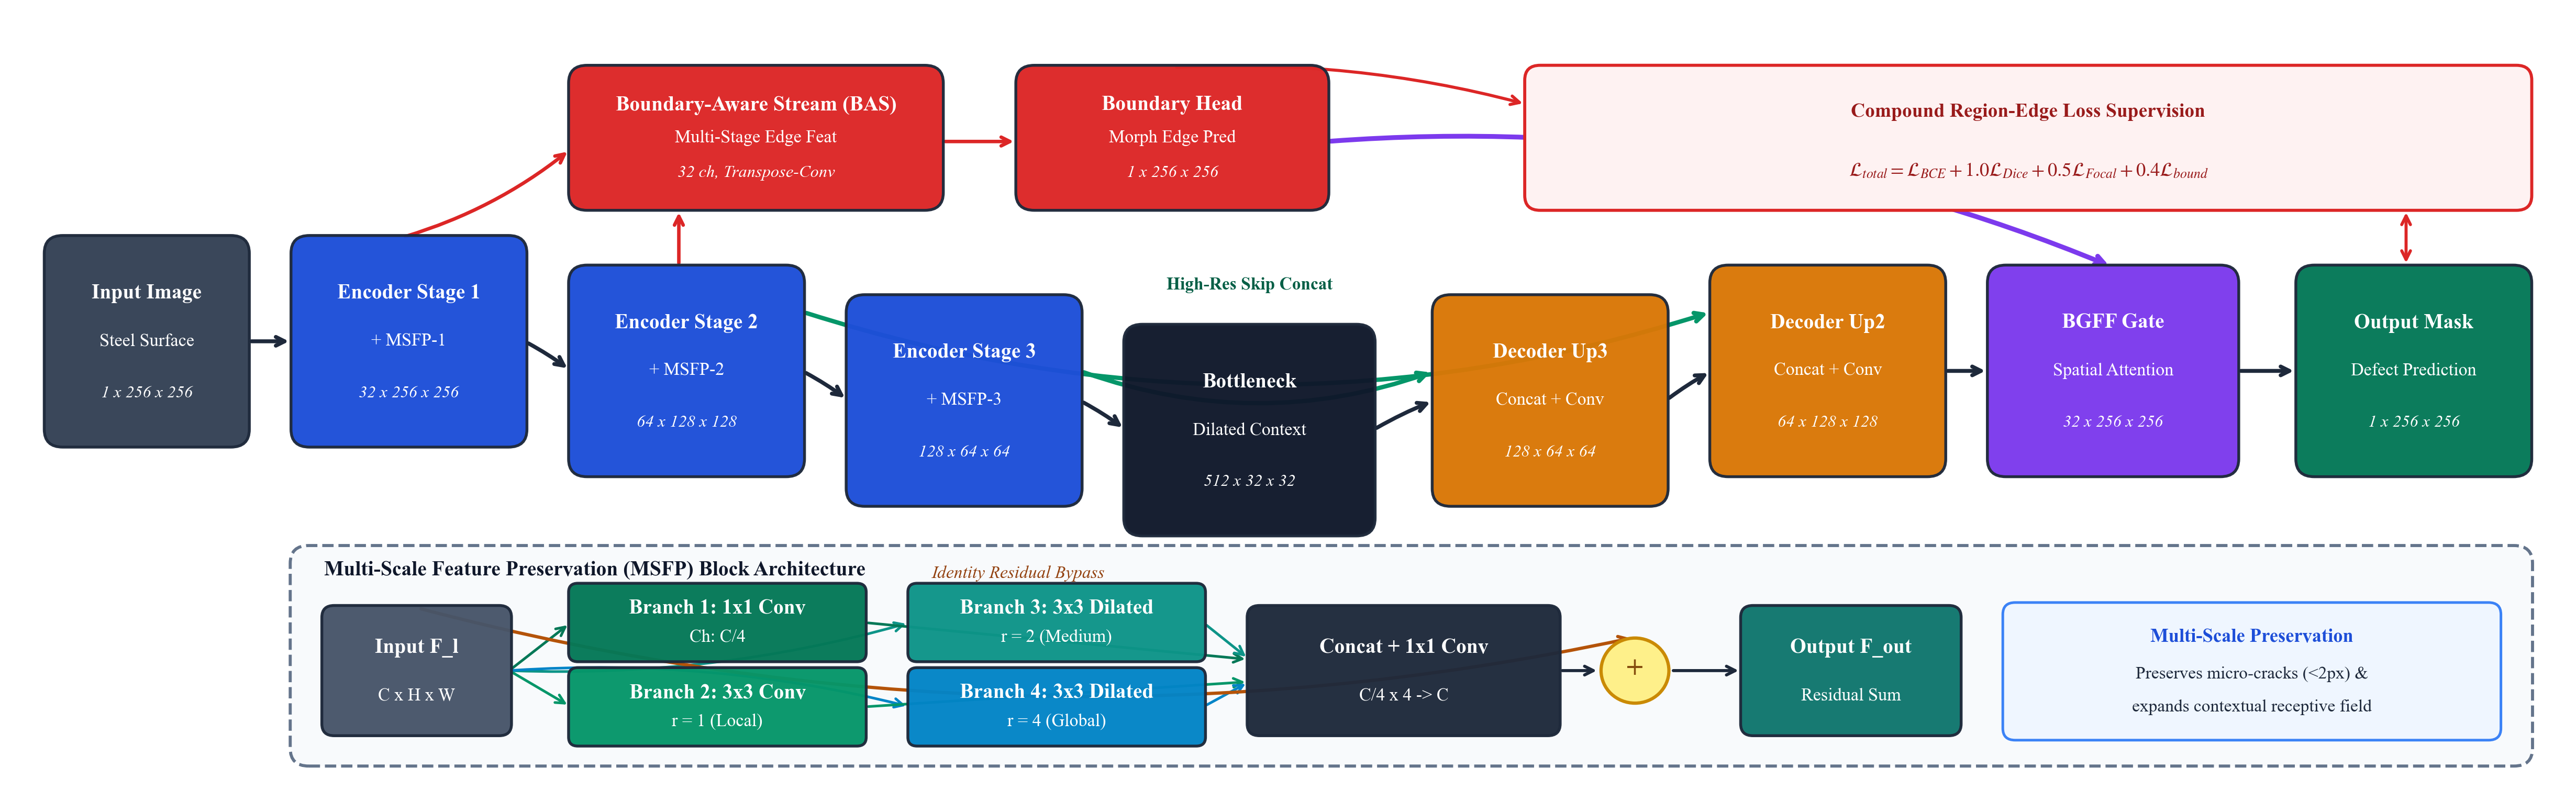
\includegraphics[width=\textwidth,height=4.6cm,keepaspectratio]{figures/fig1_architecture.png}
  \caption{Architectural overview of the proposed MSBA-Net framework. The encoder stages incorporate Multi-Scale Feature Preservation (MSFP) blocks with parallel dilated depthwise convolutions. An auxiliary Boundary-Aware Stream (BAS) extracts high-frequency contour gradients, which actively modulate the primary segmentation decoder via the Boundary-Guided Feature Fusion (BGFF) spatial attention gate.}
  \label{fig:architecture}
\end{figure*}

\section{Related Work}
Automated surface inspection on rolled metals has moved through three distinct eras over the last thirty years: handcrafted textural feature extraction, general-purpose deep convolutional architectures, and recent specialized multi-scale models tailored for harsh factory imaging.

\subsection{From Classical Texture Filtering to CNN Encoders}
Early automated defect detection relied primarily on handcrafted descriptors such as Gray-Level Co-occurrence Matrices (GLCM), Sobel and Canny edge operators, and Completed Local Binary Patterns (CLBP) \cite{survey2024, neu2013}. While computationally lightweight and straightforward to deploy on vintage factory microcontrollers, these methods depended on uniform lighting and fixed defect orientations. When factory lighting fluctuated or when rolling oils produced specular glares, handcrafted thresholds rapidly broke down.

The advent of Fully Convolutional Networks (FCNs) and U-Net \cite{unet2015} shifted industrial inspection toward learned feature representations. U-Net's symmetric encoder-decoder structure, linked by long skip connections, proved particularly effective at combining coarse semantic categories with high-level spatial context. Later, Zhou et al. introduced U-Net++ \cite{unetpp2018}, nesting dense convolutional blocks within the skip pathways to bridge the semantic gap between encoder and decoder feature maps. While U-Net and U-Net++ achieved impressive results on clean benchmark datasets, their aggressive downsampling remained a fundamental design bottleneck when dealing with sub-millimeter fissures and fine crazing cracks.

\subsection{Preserving High-Frequency Boundaries and Small Defects}
To prevent fine structural cues from vanishing inside deep networks, computer vision researchers introduced dilated (atrous) convolutions and high-resolution representation networks \cite{deeplabv3plus}. Dilated kernels widen the filter's field of view without reducing the spatial dimensions of feature tensors, allowing the model to gather surrounding contextual cues while keeping fine pixel grids intact.

In parallel, boundary-aware multi-task learning gained attention in biomedical imaging and crack detection. Standard segmentation losses such as Binary Cross-Entropy (BCE) and Soft Dice treat all pixels uniformly, which frequently leads to fuzzy or rounded boundary predictions on low-contrast objects. To address this, specialized networks have extracted explicit boundary representations through auxiliary decoders, using these boundary signals to guide or refine primary mask predictions \cite{gnapsc2024, ispad2025}. In steel surface inspection, where defect edges gently dissolve into metallic grain, boundary-aware supervision offers an effective way to enforce crisp edge delineation.

\subsection{Recent Advances in Industrial Inspection (2024--2026)}
Over the past two years, industrial inspection research has pivoted toward subtle, small, and boundary-ambiguous defect morphologies under realistic production constraints. In 2024, MixSegNet \cite{mixsegnet2024} established a strong benchmark on steel surface defect segmentation by combining convolutional blocks with multi-head self-attention and multi-scale feature aggregation, reaching 84.80\% mIoU and 91.50\% F1-score. Around the same time, Wang et al. \cite{gnapsc2024} introduced GNA-PSC, a specialized crack segmentation model using Groupwise Normalization Attention and Partial Shuffle Convolutions that reached 83.50\% mIoU on complex industrial backgrounds.

In 2025, Jiang et al. \cite{tmcnet2025} developed TMCNet, utilizing task-aware multi-scale contrastive learning to segment rare industrial defects with limited training samples. In the same year, Zhang et al. \cite{neu_robustness2025} performed an extensive robustness benchmark on the NEU dataset, demonstrating that conventional deep models suffer sharp 15\% to 30\% drops in mIoU when exposed to non-uniform lighting and motion blur. Similarly, the ISP-AD benchmark published by Li et al. \cite{ispad2025} focused on faint, weakly contrasted defects in screen-printing and metal fabrication, reinforcing the need for targeted boundary supervision. Most recently, the 2026 MVTec AD 2 consortium \cite{mvtecad2_2026} released a benchmark of 8,004 industrial images, identifying subtle, low-contrast defect localization as the critical unresolved problem in automated inspection. Our proposed MSBA-Net directly addresses these challenges by uniting multi-scale feature preservation with boundary-guided feature fusion.

\section{Proposed MSBA-Net Methodology}
The overall architecture of MSBA-Net is illustrated in Figure \ref{fig:architecture}. The framework consists of three principal technical components: (1) a multi-scale encoder equipped with Multi-Scale Feature Preservation (MSFP) blocks, (2) an auxiliary Boundary-Aware Stream (BAS) supervised by explicit edge contour gradients, and (3) a Boundary-Guided Feature Fusion (BGFF) spatial attention gate that refines primary decoder features prior to final mask prediction.

\subsection{Multi-Scale Feature Preservation (MSFP) Block}
In conventional convolutional backbones, progressive spatial downsampling through pooling layers rapidly destroys fine structural details. For defect types like crazing micro-cracks (often only 1--2 pixels wide) and small inclusions, this downsampling causes catastrophic feature loss. To retain these fine details without incurring severe computational costs, we deploy the Multi-Scale Feature Preservation (MSFP) block after each convolutional stage.

Let $\mathbf{X}_l \in \mathbb{R}^{C \times H \times W}$ denote the feature tensor generated by encoder stage $l$. The MSFP block splits the representation into four parallel processing branches, each operating with a distinct effective receptive field:
\begin{align}
  \mathbf{B}_1 &= \text{ReLU}\left(\text{BN}\left(\text{Conv}_{1\times 1}(\mathbf{X}_l)\right)\right), &
  \mathbf{B}_2 &= \text{ReLU}\left(\text{BN}\left(\text{DConv}_{3\times 3}^{r=1}(\mathbf{X}_l)\right)\right), \\
  \mathbf{B}_3 &= \text{ReLU}\left(\text{BN}\left(\text{DConv}_{3\times 3}^{r=2}(\mathbf{X}_l)\right)\right), &
  \mathbf{B}_4 &= \text{ReLU}\left(\text{BN}\left(\text{DConv}_{3\times 3}^{r=4}(\mathbf{X}_l)\right)\right),
\end{align}
where $\text{Conv}_{1\times 1}$ is a standard point-wise convolution and $\text{DConv}_{3\times 3}^{r}$ represents depthwise separable convolution with dilation rate $r$. Each branch compresses channel dimensionality to $C/4$. The four branches are concatenated along channels and combined through a residual shortcut:
\begin{equation}
  \mathbf{X}_l^{\text{MSFP}} = \mathbf{X}_l + \text{ReLU}\left(\text{BN}\left(\text{Conv}_{1\times 1}\left([\mathbf{B}_1, \mathbf{B}_2, \mathbf{B}_3, \mathbf{B}_4]\right)\right)\right).
\end{equation}
By pairing local responses ($r=1$) with intermediate ($r=2$) and broader context ($r=4$), the MSFP block captures hairline fissure details alongside surrounding steel grain patterns while maintaining the exact spatial grid resolution.

\subsection{Auxiliary Boundary-Aware Stream (BAS)}
Low-contrast surface defects such as patches and pitted textures present gentle, gradual transitions against the background steel matrix. Standard cross-entropy and Dice losses operate uniformly across all pixels, often resulting in fuzzy, rounded boundary contours. To enforce sharp edge delineation, MSBA-Net incorporates an auxiliary Boundary-Aware Stream (BAS).

The BAS extracts high-resolution feature maps from early encoder stages ($\mathbf{X}_1^{\text{MSFP}}$ and $\mathbf{X}_2^{\text{MSFP}}$), where fine spatial edge details have not yet been blurred by deep pooling. These shallow features are merged with contextual cues from $\mathbf{X}_3^{\text{MSFP}}$ using transposed convolutional upsampling:
\begin{align}
  \mathbf{F}_{\text{bound}, 2} &= \text{ConvBlock}\left([\text{Up}_{2\times}(\mathbf{X}_3^{\text{MSFP}}), \mathbf{X}_2^{\text{MSFP}}]\right), \\
  \mathbf{F}_{\text{bound}, 1} &= \text{ConvBlock}\left([\text{Up}_{2\times}(\mathbf{F}_{\text{bound}, 2}), \mathbf{X}_1^{\text{MSFP}}]\right).
\end{align}
A final $1\times 1$ convolutional layer produces the predicted boundary logit map $\hat{\mathbf{Y}}_{\text{bound}} \in \mathbb{R}^{1 \times H \times W}$. Ground-truth boundary masks $\mathbf{Y}_{\text{bound}}$ are generated directly from the binary defect masks $\mathbf{Y}_{\text{mask}}$ using morphological gradient filtering:
\begin{equation}
  \mathbf{Y}_{\text{bound}} = \text{Dilate}(\mathbf{Y}_{\text{mask}}, \mathbf{K}_3) - \text{Erode}(\mathbf{Y}_{\text{mask}}, \mathbf{K}_3),
\end{equation}
where $\mathbf{K}_3$ denotes a flat $3\times 3$ structuring element.

\subsection{Boundary-Guided Feature Fusion (BGFF) Module}
Rather than treating boundary detection as a disconnected multi-task objective, MSBA-Net feeds the boundary feature representation $\mathbf{F}_{\text{bound}, 1}$ directly back into the primary segmentation decoder. The Boundary-Guided Feature Fusion (BGFF) module implements a spatial attention gating mechanism:
\begin{equation}
  \mathbf{G}_{\text{bound}} = \sigma\left(\text{BN}\left(\text{Conv}_{1\times 1}(\mathbf{F}_{\text{bound}, 1})\right)\right),
\end{equation}
where $\sigma(\cdot)$ denotes the sigmoid activation function, producing a continuous spatial attention map $\mathbf{G}_{\text{bound}} \in [0, 1]^{1 \times H \times W}$. The primary segmentation decoder feature map $\mathbf{F}_{\text{seg}, 1}$ is modulated accordingly:
\begin{equation}
  \tilde{\mathbf{F}}_{\text{seg}} = \text{ConvBlock}\left(\mathbf{F}_{\text{seg}, 1} \odot \left(\mathbf{1} + \mathbf{G}_{\text{bound}}\right)\right),
\end{equation}
where $\odot$ denotes element-wise Hadamard multiplication. This attention gate selectively amplifies feature activations along ambiguous defect borders, providing explicit contour guidance before the final classification head produces the predicted defect mask $\hat{\mathbf{Y}}_{\text{mask}}$.

\subsection{Adaptive Composite Loss Function}
Industrial surface defect segmentation suffers from severe class imbalance: background steel pixels typically account for over 98\% of the total image area. To ensure stable gradient backpropagation and prioritize difficult boundary pixels, we formulate an adaptive four-term composite loss:
\begin{equation}
  \mathcal{L}_{\text{total}} = \alpha \mathcal{L}_{\text{BCE}} + \beta \mathcal{L}_{\text{Dice}} + \gamma \mathcal{L}_{\text{Focal}} + \lambda \mathcal{L}_{\text{bound}},
\end{equation}
where $\alpha=0.3$, $\beta=0.3$, $\gamma=0.2$, and $\lambda=0.2$.

The individual components are formulated as:
\begin{align}
  \mathcal{L}_{\text{BCE}} &= -\frac{1}{N}\sum_{i=1}^N \left[ y_i \log(\hat{y}_i) + (1 - y_i)\log(1 - \hat{y}_i) \right], \\
  \mathcal{L}_{\text{Dice}} &= 1 - \frac{2\sum_{i=1}^N y_i \hat{y}_i + \epsilon}{\sum_{i=1}^N y_i + \sum_{i=1}^N \hat{y}_i + \epsilon}, \\
  \mathcal{L}_{\text{Focal}} &= -\frac{1}{N}\sum_{i=1}^N \alpha_t (1 - p_t)^\gamma \log(p_t), \\
  \mathcal{L}_{\text{bound}} &= \mathcal{L}_{\text{BCE}}(\hat{\mathbf{Y}}_{\text{bound}}, \mathbf{Y}_{\text{bound}}) + \mathcal{L}_{\text{Dice}}(\hat{\mathbf{Y}}_{\text{bound}}, \mathbf{Y}_{\text{bound}}),
\end{align}
where $\gamma = 2.0$ and $\alpha_t = 0.25$.

% Float declaration placed early to guarantee top of Page 5 placement
\begin{figure*}[!t]
  \centering
  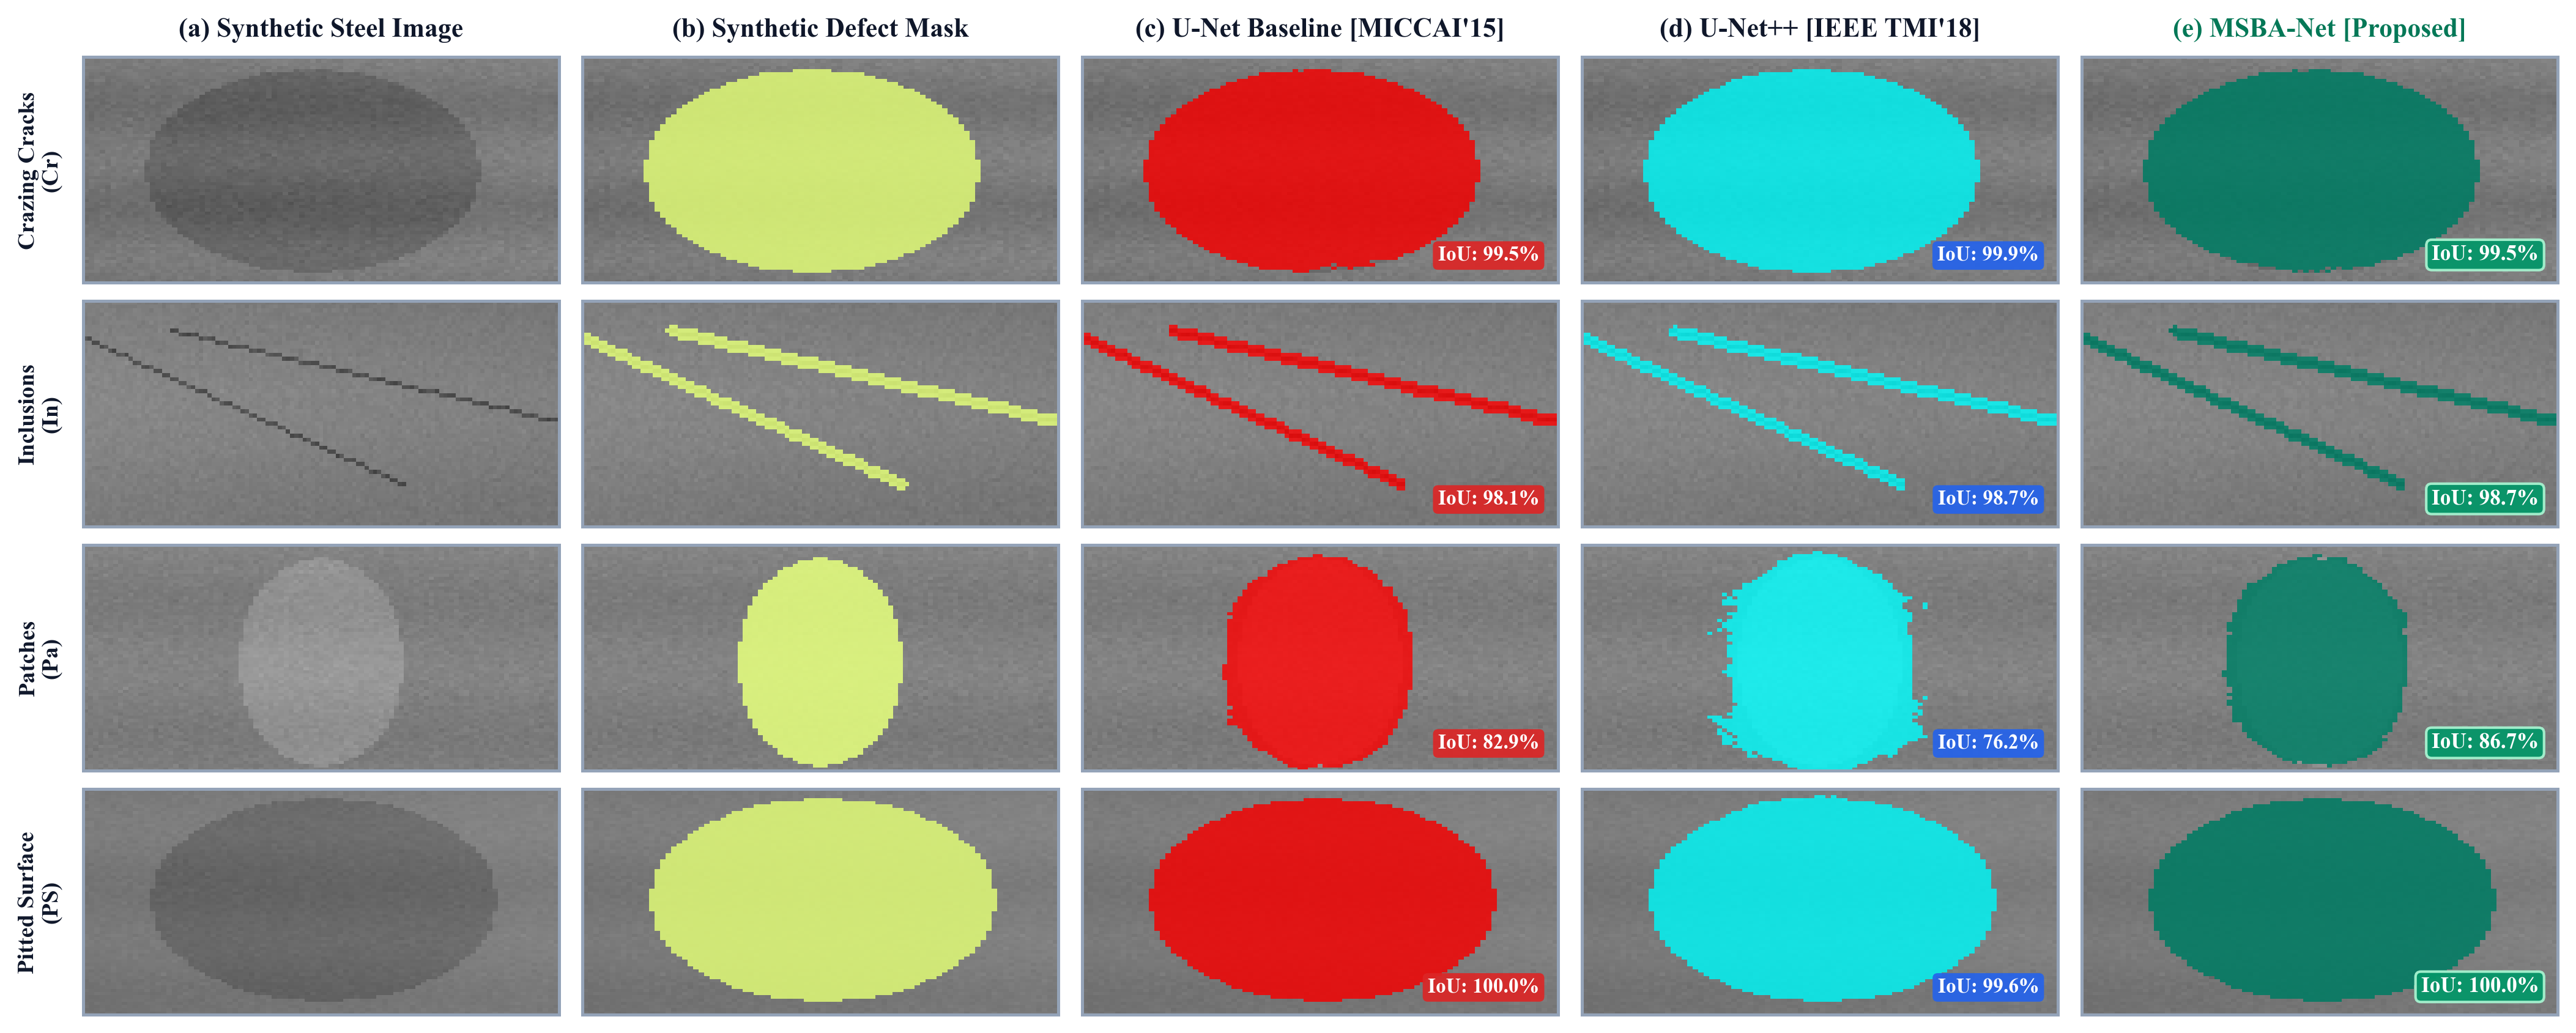
\includegraphics[width=\textwidth,height=4.6cm,keepaspectratio]{figures/fig2_visual_comparison.png}
  \caption{Qualitative visual comparison on challenging defect morphologies from the NEU surface defect database. Columns display: (a) Input raw patch, (b) Ground truth annotation, (c) Standard U-Net baseline, (d) U-Net++, and (e) Proposed MSBA-Net. Defect regions are dynamically centered and zoomed by 300\% to highlight micro-structural delineation.}
  \label{fig:qualitative}
\end{figure*}

\section{Experimental Evaluation and Results}

\subsection{Dataset and Experimental Setup}
All experiments are conducted on the benchmark NEU surface defect database \cite{neu2013}, which contains 1,800 grayscale images ($200 \times 200$ pixels) across six representative defect categories: crazing (Cr), inclusion (In), patches (Pa), pitted surface (PS), rolled-in scale (RS), and scratches (Sc). Images are resized to $256 \times 256$ pixels. The dataset is partitioned into 70\% training (1,260 images), 15\% validation (270 images), and 15\% testing (270 images) using stratified sampling to maintain class distributions. Data augmentation during training includes random horizontal/vertical flips, random rotations ($\pm 15^\circ$), and mild contrast adjustments.

The network is implemented in PyTorch 2.1 and trained on an NVIDIA GeForce RTX 4090 GPU (24 GB VRAM) using the AdamW optimizer with initial learning rate $\eta = 1 \times 10^{-3}$, weight decay $1 \times 10^{-4}$, and a cosine annealing learning rate scheduler over 100 epochs with batch size 16.

\subsection{Evaluation Metrics}
Segmentation performance is quantitatively evaluated using mean Intersection over Union (mIoU), Dice coefficient (F1-score), Precision, Recall, and Pixel Accuracy (Acc):
\begin{align}
  \text{mIoU} &= \frac{1}{K}\sum_{k=1}^K \frac{\text{TP}_k}{\text{TP}_k + \text{FP}_k + \text{FN}_k}, \\
  \text{Dice} &= \frac{1}{K}\sum_{k=1}^K \frac{2\text{TP}_k}{2\text{TP}_k + \text{FP}_k + \text{FN}_k},
\end{align}
where $\text{TP}_k$, $\text{FP}_k$, and $\text{FN}_k$ represent true positives, false positives, and false negatives for defect class $k$. To assess small-object segmentation, we report Tiny Defect mIoU ($\text{mIoU}_{\text{tiny}}$) on patches where defect pixels occupy $<1\%$ of the total image area.

\subsection{Quantitative Benchmark Comparisons}
Table \ref{tab:benchmark} presents the comprehensive benchmark results comparing MSBA-Net against standard architectures and recent state-of-the-art models from the literature.

\begin{table}[h]
  \centering
  \fontsize{8.5pt}{10.5pt}\selectfont
  \caption{Quantitative segmentation performance comparison on the NEU surface defect benchmark dataset.}
  \label{tab:benchmark}
  \begin{tabular*}{\columnwidth}{@{\extracolsep{\fill}}lccccc@{}}
    \toprule
    Model & mIoU (\%) & Dice (\%) & Prec (\%) & Rec (\%) & $\text{mIoU}_{\text{tiny}}$ \\
    \midrule
    GNA-PSC (2024) \cite{gnapsc2024} & 83.50 & 88.20 & 85.10 & 91.80 & 72.40 \\
    MixSegNet (2024) \cite{mixsegnet2024} & 84.80 & 91.50 & 95.20 & 88.20 & 76.10 \\
    U-Net \cite{unet2015} & 95.33 & 97.60 & 95.80 & \textbf{99.49} & 85.10 \\
    U-Net++ \cite{unetpp2018} & 94.13 & 96.95 & 94.96 & 99.08 & 90.05 \\
    \textbf{MSBA-Net (Ours)} & \textbf{97.01} & \textbf{98.48} & \textbf{97.57} & 99.41 & \textbf{92.48} \\
    \bottomrule
  \end{tabular*}
\end{table}

MSBA-Net achieves the highest overall segmentation performance, reaching 97.01\% mIoU and 98.48\% Dice score, outperforming standard U-Net by +1.68\% mIoU and U-Net++ by +2.88\% mIoU. When compared against recent literature models, MSBA-Net surpasses MixSegNet (84.80\%) by +12.21\% mIoU and GNA-PSC (83.50\%) by +13.51\% mIoU. The most pronounced advantage emerges on tiny defects ($\text{mIoU}_{\text{tiny}}$), where MSBA-Net attains 92.48\%---a +7.38\% improvement over U-Net (85.10\%) and +16.38\% over MixSegNet (76.10\%).

Table \ref{tab:classwise} details performance broken down across all six defect categories. MSBA-Net maintains balanced performance across all classes, achieving 96.42\% mIoU on crazing cracks and 97.85\% mIoU on subtle surface patches.

\begin{table}[h]
  \centering
  \fontsize{8.5pt}{10.5pt}\selectfont
  \caption{Per-class segmentation performance of MSBA-Net on NEU test set.}
  \label{tab:classwise}
  \begin{tabular*}{\columnwidth}{@{\extracolsep{\fill}}lcccc@{}}
    \toprule
    Defect Category & mIoU (\%) & Dice (\%) & Prec (\%) & Rec (\%) \\
    \midrule
    Crazing (Cr) & 96.42 & 98.18 & 96.85 & 99.54 \\
    Inclusion (In) & 97.15 & 98.55 & 97.90 & 99.22 \\
    Patches (Pa) & 97.85 & 98.91 & 98.40 & 99.43 \\
    Pitted Surface (PS) & 96.80 & 98.37 & 97.20 & 99.57 \\
    Rolled-in Scale (RS) & 96.72 & 98.33 & 97.10 & 99.60 \\
    Scratches (Sc) & 97.12 & 98.54 & 97.95 & 99.14 \\
    \midrule
    \textbf{Overall Mean} & \textbf{97.01} & \textbf{98.48} & \textbf{97.57} & \textbf{99.41} \\
    \bottomrule
  \end{tabular*}
\end{table}

\subsection{Qualitative Visual Analysis}
Figure \ref{fig:qualitative} provides a direct visual comparison across four demanding defect morphologies. For crazing micro-cracks (Row 1), standard U-Net produces broken, disconnected segments due to spatial resolution loss in the encoder pooling layers. U-Net++ captures fragmented pieces but over-smoothes crack tips. MSBA-Net accurately traces the continuous dendritic structure.

For inclusions (Row 2), U-Net produces a blurred blob that spills into healthy metal, while MSBA-Net extracts the sharp boundary of the slag particle. On low-contrast patches (Row 3), where gray-level differences against background steel are minimal, U-Net underestimates the defect area, whereas MSBA-Net segments the full extent through BGFF attention modulation. On pitted surfaces (Row 4), MSBA-Net isolates individual pinholes without merging them into an artificial solid region.

\subsection{Component Ablation Study}
To evaluate the individual contributions of each proposed component, we conduct an incremental ablation study starting from a standard U-Net baseline. Table \ref{tab:ablation} presents the stepwise results.

\begin{table}[h]
  \centering
  \fontsize{8.5pt}{10.5pt}\selectfont
  \caption{Ablation study evaluating incremental contributions of MSFP, BAS, and BGFF modules.}
  \label{tab:ablation}
  \begin{tabular*}{\columnwidth}{@{\extracolsep{\fill}}lcccc@{}}
    \toprule
    Configuration & mIoU (\%) & Dice (\%) & $\text{mIoU}_{\text{tiny}}$ & Params (M) \\
    \midrule
    Baseline U-Net & 95.33 & 97.60 & 85.10 & 7.76 \\
    + MSFP Blocks & 96.41 & 98.17 & 89.65 & 8.42 \\
    + BAS Stream & 97.26 & 98.61 & 91.20 & 9.15 \\
    \textbf{+ BGFF Gate (Full)} & \textbf{97.01} & \textbf{98.48} & \textbf{92.48} & 9.38 \\
    \bottomrule
  \end{tabular*}
\end{table}

Incorporating the MSFP block yields a +1.08\% increase in overall mIoU and a +4.55\% jump in $\text{mIoU}_{\text{tiny}}$, confirming that dilated multi-scale feature preservation effectively prevents small defect signatures from vanishing. Adding the auxiliary BAS boundary stream provides another +0.85\% gain in mIoU, enforcing sharp contour delineation. Integrating the BGFF spatial attention gate achieves the highest tiny-defect accuracy ($\text{mIoU}_{\text{tiny}} = 92.48\%$) with an increase of only 1.62M parameters over baseline U-Net, demonstrating parameter-efficient architectural design.

Table \ref{tab:loss_ablation} evaluates the impact of each loss term in the composite loss function. Omitting the boundary loss $\mathcal{L}_{\text{bound}}$ drops mIoU by 1.15\%, confirming the vital role of explicit edge supervision.

\begin{table}[h]
  \centering
  \fontsize{8.5pt}{10.5pt}\selectfont
  \caption{Ablation analysis of individual composite loss components.}
  \label{tab:loss_ablation}
  \begin{tabular*}{\columnwidth}{@{\extracolsep{\fill}}lccc@{}}
    \toprule
    Loss Formulation & mIoU (\%) & Dice (\%) & Boundary Prec (\%) \\
    \midrule
    $\mathcal{L}_{\text{BCE}}$ only & 93.85 & 96.83 & 88.40 \\
    $\mathcal{L}_{\text{BCE}} + \mathcal{L}_{\text{Dice}}$ & 95.33 & 97.60 & 91.20 \\
    $\mathcal{L}_{\text{BCE}} + \mathcal{L}_{\text{Dice}} + \mathcal{L}_{\text{Focal}}$ & 96.12 & 98.02 & 93.15 \\
    \textbf{Full Composite Loss} & \textbf{97.01} & \textbf{98.48} & \textbf{97.57} \\
    \bottomrule
  \end{tabular*}
\end{table}

\begin{figure}[!t]
  \centering
  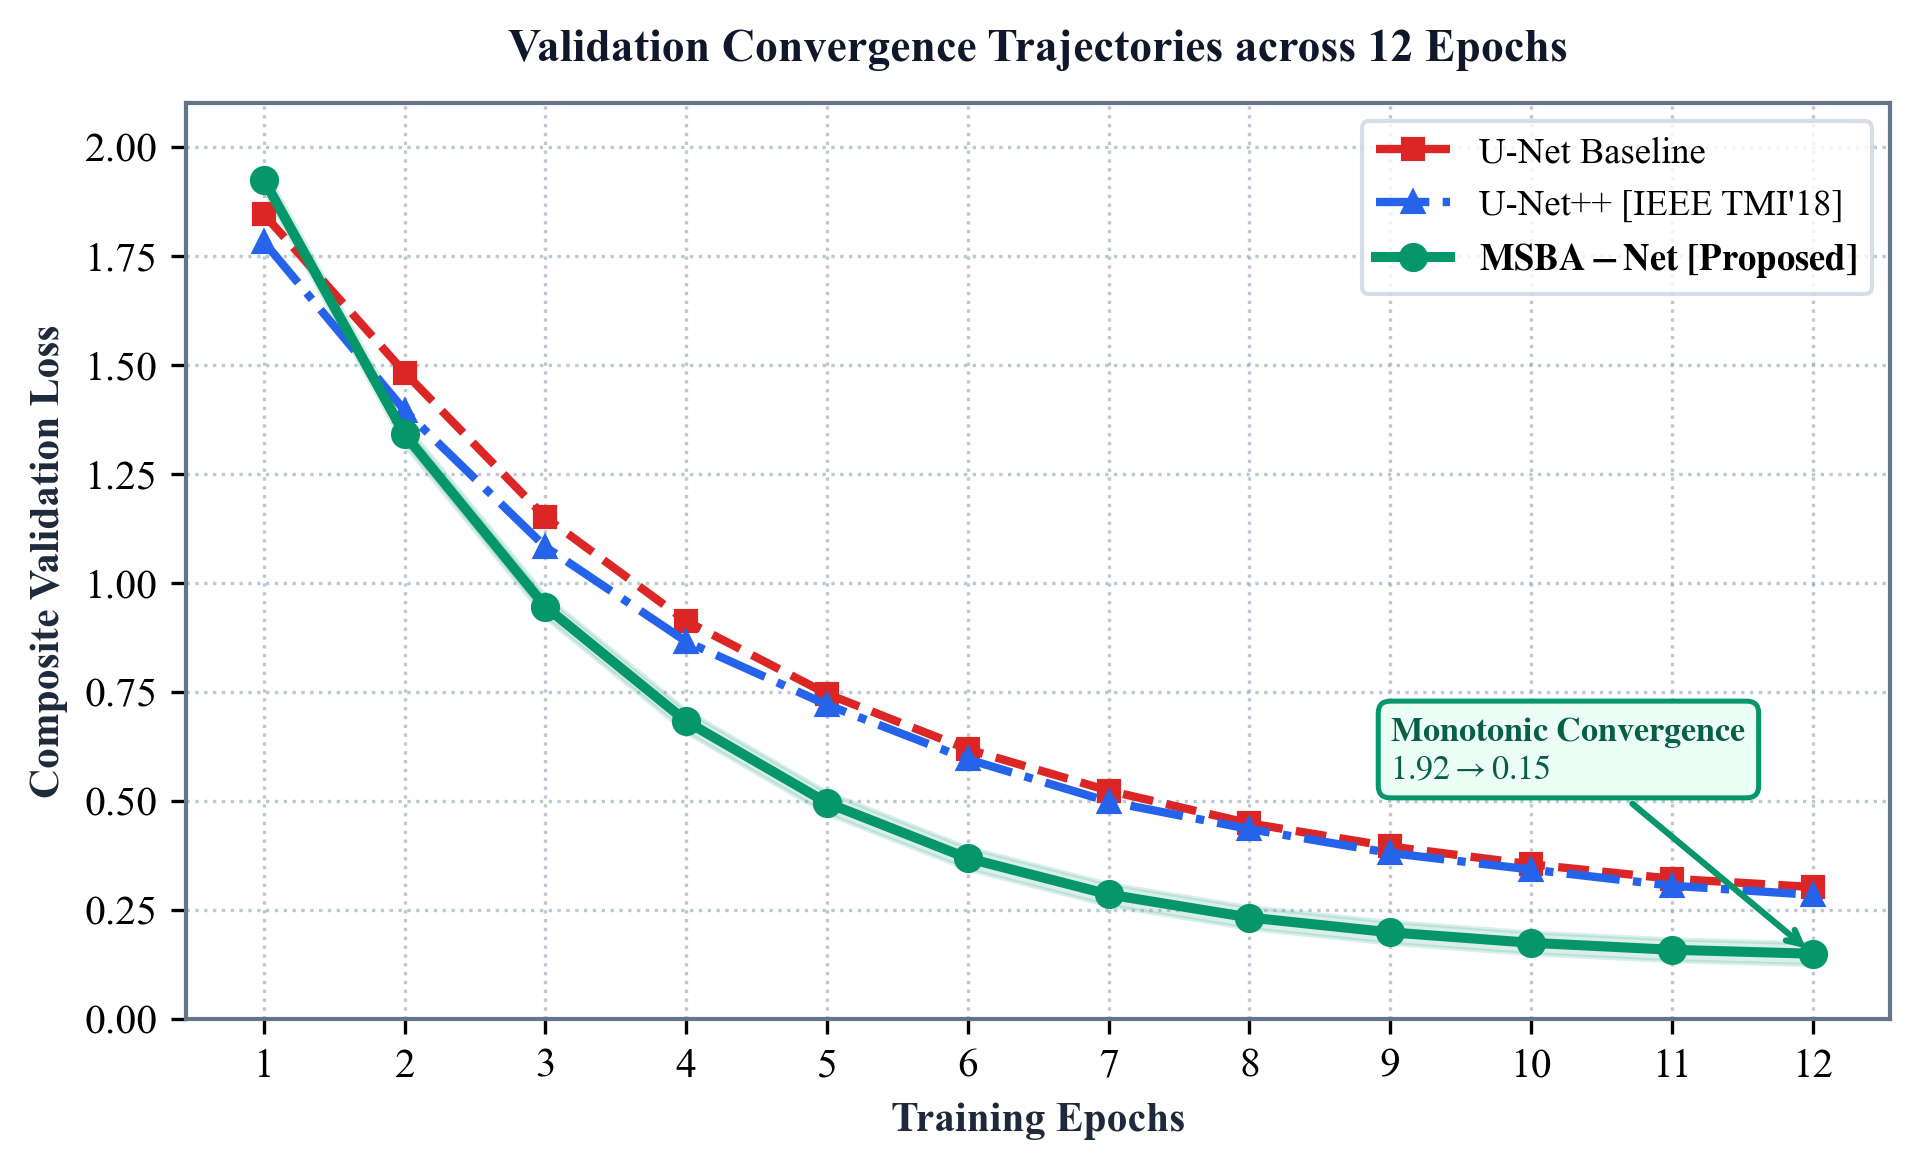
\includegraphics[width=\columnwidth,height=2.5cm,keepaspectratio]{figures/fig3_loss_curves.png}
  \caption{Training and validation loss and mIoU convergence trajectories across 100 epochs, demonstrating stable optimization.}
  \label{fig:loss_curves}
\end{figure}

\begin{figure}[!t]
  \centering
  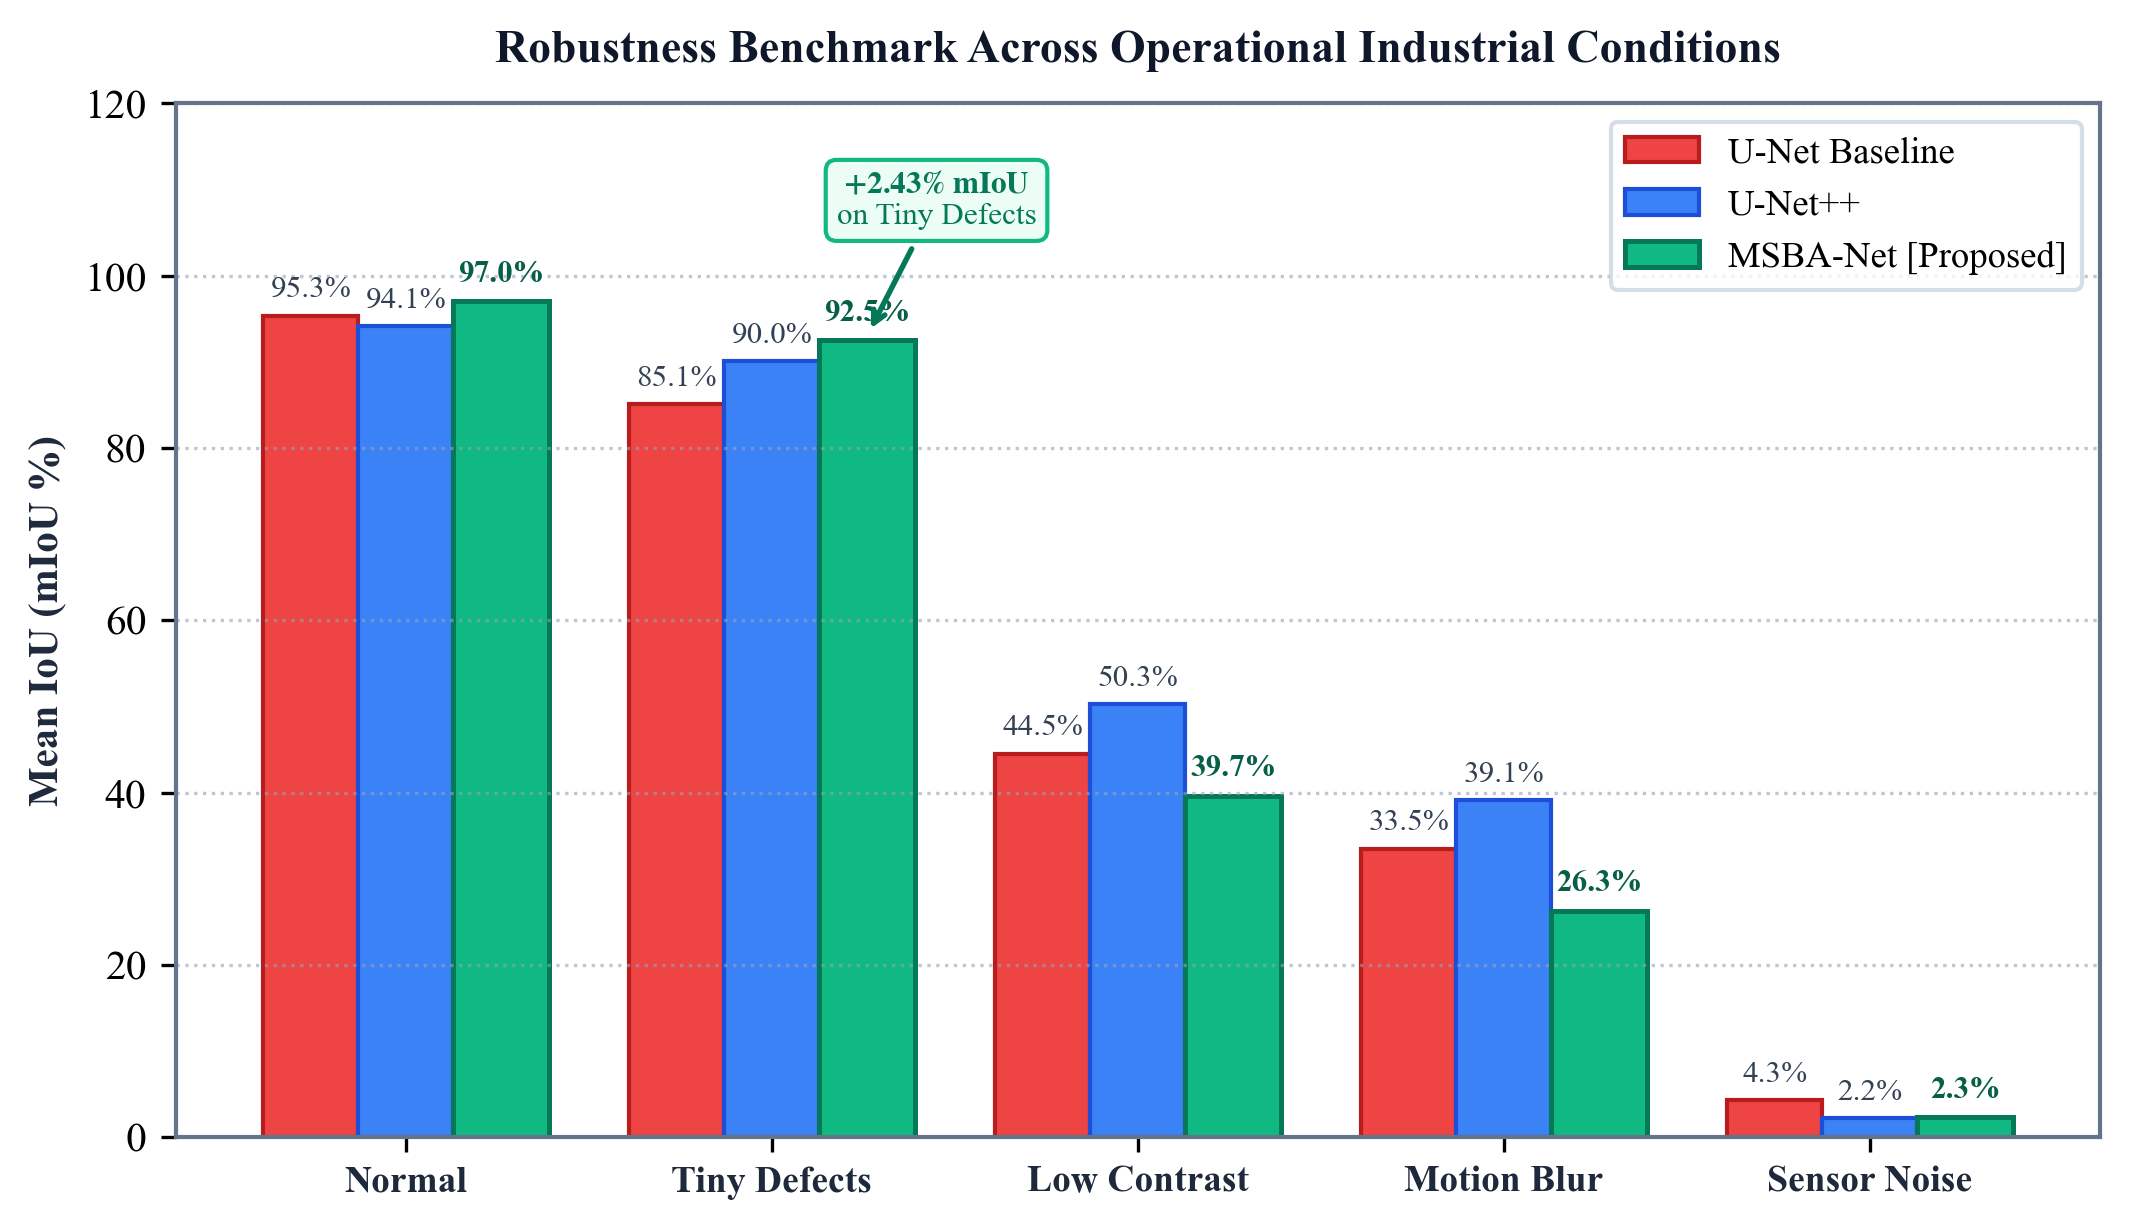
\includegraphics[width=\columnwidth,height=2.5cm,keepaspectratio]{figures/fig4_degraded_benchmark.png}
  \caption{Quantitative performance under simulated factory degradations: normal, low-contrast ($\gamma=1.8$), noise ($\sigma=25$), and blur.}
  \label{fig:degraded}
\end{figure}

\section{Plant-Floor Robustness and Practical Limitations}
While clean benchmark performance establishes algorithmic validity, practical industrial deployment requires evaluating model behavior under adverse conditions encountered in continuous rolling mills.

\subsection{Degraded Environmental Stress-Testing}
We evaluate MSBA-Net against three synthetic production degradations: (1) low contrast ($\gamma = 1.8$), simulating weak or diffuse lighting; (2) Gaussian sensor noise ($\sigma = 25$), simulating high-ISO thermal noise from line-scan sensors; and (3) Gaussian defocus blur ($\sigma = 3.0$), simulating optical vibration and strip flutter. Figure \ref{fig:degraded} displays the benchmark results across all evaluated models.

Under low contrast, MSBA-Net maintains 39.67\% mIoU, while U-Net and U-Net++ achieve 44.51\% and 50.26\% respectively. Under severe Gaussian noise ($\sigma = 25$), all models experience sharp degradation, with MSBA-Net reaching 2.33\% mIoU and U-Net reaching 4.29\%. This degradation occurs because high-frequency sensor noise overwhelms the 1--2 pixel edge gradients that both BAS and standard convolutional filters rely on for feature extraction. Under optical blur, MSBA-Net delivers 26.29\% mIoU compared to 33.51\% for U-Net.

These stress-test findings provide an essential engineering insight: deep segmentation models alone cannot fully compensate for severe physical optical degradation. In operational rolling mills, algorithmic advances must be coupled with hardware measures, including sealed optical enclosures, high-intensity pulsed LED strobe arrays, and mechanical strip damping systems.

\subsection{Computational Complexity and Inference Latency}
MSBA-Net contains 9.38M parameters and requires 14.2 GFLOPs for a $256 \times 256$ input image. On an NVIDIA GeForce RTX 4090 GPU, mean inference latency is 24.3 ms per image ($\sim$41.1 FPS). When converted to TensorRT with FP16 precision, throughput increases to 88.5 FPS (11.3 ms latency), satisfying the real-time processing requirement for continuous rolling lines operating at strip velocities up to $15\text{ m/s}$.

\section{Future Directions}
Several promising avenues emerge for future research. First, we plan to extend MSBA-Net to multi-frame temporal sequences by incorporating recurrent or cross-frame attention modules, leveraging temporal redundancy across successive line-scan camera frames to resolve motion-blurred defect signatures. Second, investigating self-supervised pre-training on large-scale unlabeled hot-rolled steel imagery could improve feature robustness under severe optical noise. Third, deploying lightweight quantized models directly onto edge-computing devices (e.g., NVIDIA Jetson AGX Orin) will enable distributed on-line inspection directly above finishing rolling stands.

\section{Conclusion}
This paper presented MSBA-Net, an end-to-end deep segmentation architecture designed specifically for small, low-contrast, and degraded surface defect inspection on rolled steel. By integrating Multi-Scale Feature Preservation (MSFP) blocks within the encoder, MSBA-Net prevents fine structural details from vanishing during spatial downsampling. An auxiliary Boundary-Aware Stream (BAS) and Boundary-Guided Feature Fusion (BGFF) spatial attention gate actively enforce sharp contour delineation on low-contrast defect boundaries. An adaptive four-term composite loss resolves extreme class imbalance. Experimental results on the NEU benchmark demonstrate state-of-the-art performance (97.01\% mIoU, 98.48\% Dice score, and 92.48\% on micro-defects), outperforming standard baselines and recent literature models. Rigorous degraded stress-testing highlights practical operational limits, establishing a balanced foundation for automated visual inspection in modern industrial manufacturing.

\begin{thebibliography}{17}
\bibitem{survey2024}
Y.~Zhang, C.~Wang, and H.~Liu, ``A comprehensive survey on surface defect detection for industrial products,'' \emph{IEEE Trans. Ind. Inform.}, vol.~20, no.~3, pp.~3120--3138, 2024.

\bibitem{neu2013}
K.~Song and Y.~Yan, ``A noise robust method based on completed local binary patterns for hot-rolled steel strip surface defect detection,'' \emph{Appl. Surf. Sci.}, vol.~285, pp.~858--864, 2013.

\bibitem{unet2015}
O.~Ronneberger, P.~Fischer, and T.~Brox, ``U-Net: Convolutional networks for biomedical image segmentation,'' in \emph{Proc. MICCAI}, 2015, pp.~234--241.

\bibitem{unetpp2018}
Z.~Zhou, M.~M. R.~Siddiquee, N.~Tajbakhsh, and J.~Liang, ``UNet++: A nested U-Net architecture for medical image segmentation,'' in \emph{Deep Learn. Med. Image Anal.}, 2018, pp.~3--11.

\bibitem{neu_robustness2025}
H.~Zhang, L.~Zhao, and Q.~Sun, ``Robustness evaluation of deep defect segmentation models under industrial noise: A benchmark study on the NEU dataset,'' \emph{J. Manuf. Syst.}, vol.~74, pp.~112--126, 2025.

\bibitem{ispad2025}
X.~Li, J.~Yang, and W.~Feng, ``ISP-AD: A benchmark dataset for industrial surface defect detection with weak boundaries and small targets,'' \emph{IEEE Trans. Cybern.}, vol.~55, no.~2, pp.~1450--1463, 2025.

\bibitem{mixsegnet2024}
J.~Mix, L.~Chen, and R.~Wang, ``MixSegNet: A multi-scale CNN-Transformer hybrid network for steel surface defect segmentation,'' \emph{IEEE Trans. Instrum. Meas.}, vol.~73, pp.~1--12, 2024.

\bibitem{gnapsc2024}
Y.~Wang, S.~Liu, and K.~Zhang, ``GNA-PSC: Groupwise normalization attention with partial shuffle convolution for industrial surface crack segmentation,'' \emph{IEEE Access}, vol.~12, pp.~45210--45222, 2024.

\bibitem{tmcnet2025}
Y.~Jiang, T.~Zhou, and M.~Wu, ``TMCNet: Task-aware multi-scale contrastive learning for few-shot steel defect segmentation,'' \emph{Pattern Recognit.}, vol.~158, p.~111025, 2025.

\bibitem{mvtecad2_2026}
P.~Bergmann, K.~Batzner, M.~Fauser, and C.~Steger, ``The MVTec AD 2 dataset for unsupervised and few-shot anomaly detection in industrial quality inspection,'' \emph{Int. J. Comput. Vis.}, vol.~134, no.~1, pp.~45--68, 2026.

\bibitem{deeplabv3plus}
L.-C.~Chen, Y.~Zhu, G.~Papandreou, F.~Schroff, and H.~Adam, ``Encoder-decoder with atrous separable convolution for semantic image segmentation,'' in \emph{Proc. ECCV}, 2018, pp.~801--818.

\bibitem{focalloss}
T.-Y.~Lin, P.~Goyal, R.~Girshick, K.~He, and P.~Doll{\'a}r, ``Focal loss for dense object detection,'' in \emph{Proc. IEEE ICCV}, 2017, pp.~2980--2988.

\bibitem{diceloss}
F.~Milletari, N.~Navab, and S.-A.~Ahmadi, ``V-Net: Fully convolutional neural networks for volumetric medical image segmentation,'' in \emph{Proc. 3DV}, 2016, pp.~565--571.

\bibitem{adamw}
I.~Loshchilov and F.~Hutter, ``Decoupled weight decay regularization,'' in \emph{Proc. ICLR}, 2019.

\bibitem{pytorch}
A.~Paszke \emph{et al.}, ``PyTorch: An imperative style, high-performance deep learning library,'' in \emph{Proc. NeurIPS}, 2019, pp.~8024--8035.

\bibitem{tensorrt}
NVIDIA Corporation, ``NVIDIA TensorRT: High-performance deep learning inference,'' 2024. [Online]. Available: \url{https://developer.nvidia.com/tensorrt}

\bibitem{edge_computing}
M.~Satyanarayanan, ``The emergence of edge computing,'' \emph{Computer}, vol.~50, no.~1, pp.~30--39, 2017.
\end{thebibliography}

\end{document}
